\documentclass[11pt,a4paper]{article}
\usepackage[a4paper,margin=2.5cm]{geometry}
\setlength{\emergencystretch}{3em}
\usepackage{graphicx}
\usepackage{booktabs}
\usepackage{amsmath}
\usepackage{xcolor}
\usepackage{caption}
\usepackage[hidelinks]{hyperref}

\graphicspath{{figures/}}
\captionsetup{font=small,labelfont=bf}

\title{\textbf{Basic Dense Matrix Multiplication in Python, Java and C:\\
A Controlled Benchmarking Study}}
\author{Alejandro Delgado Valera\\
\small BIG DATA -- Individual Assignment 1\\
\small Grado en Ciencia e Ingenier{\'i}a de Datos\\
\small Universidad de Las Palmas de Gran Canaria\\
\small \url{https://github.com/aledelgadoo/individual-assignments-bigdata}}
\date{October 7, 2026}

\begin{document}
\maketitle

\begin{abstract}
\noindent\textbf{Question:} how does matrix size $n$ affect the runtime and memory of
one straightforward $O(n^3)$ triple-loop dense matrix multiplication implemented in
Python, Java and C under identical, controlled conditions? We implement the same
$i$--$j$--$k$ algorithm in the three languages with IEEE-754 \texttt{float64}
arithmetic and byte-identical inputs (seed 42, $n \in \{10,50,100,200,500,1000,2000\}$),
and measure the isolated multiplication kernel with monotonic clocks, warm-ups,
batches of at least 0.2\,s, five repetitions per configuration, and a declared budget
of 60\,s per multiplication and 4\,GiB of memory. Across the feasible range, runtime
grows close to the cubic model (fitted exponents 3.22--3.64 for $n \ge 100$) with
large language-dependent constants: Python takes 113--169$\times$ longer than C and
Java 1.2--2.9$\times$ longer than C. Peak resident memory grows quadratically plus a
language runtime overhead. The largest feasible sizes under the budget are $n=500$
for Python (24.2\,s) and $n=1000$ for Java (5.2\,s) and C (2.3\,s); $n=2000$
exceeded the budget in all three languages and is reported as a timeout without an
invented runtime. Conclusions are scoped to these implementations, this machine and
these inputs.
\end{abstract}

\section{Introduction and objective}

Dense matrix multiplication is the canonical example for reasoning about
algorithmic complexity: the textbook triple loop performs $2n^3$ floating-point
operations, so any implementation should show roughly cubic growth with the side
length $n$~\cite{strang2016,cormen2022}. In practice the constant factors differ by
orders of magnitude between an interpreted language, a just-in-time compiled virtual
machine and ahead-of-time compiled native code, and the memory hierarchy eventually
dominates the arithmetic.

\textbf{Research question.} How does the matrix size $n$ affect the runtime and the
memory use of a basic dense matrix multiplication implemented in Python, Java and C,
under the documented execution conditions of this study?

\textbf{Hypotheses (stated before measurement).}
\begin{enumerate}
  \item[H1:] Runtime grows as $T(n) \propto n^3$ over the tested range, with
        measurable deviations at large $n$ caused by the memory hierarchy.
  \item[H2:] The constant factors are ordered Python $\gg$ Java $\approx$ C, because
        Python executes each scalar operation through the interpreter, HotSpot
        compiles Java bytecode to machine code, and C is compiled ahead of time.
  \item[H3:] Memory grows as $3 \times 8n^2$ bytes for the three \texttt{float64}
        matrices plus a per-language runtime overhead.
\end{enumerate}

The factor comparison is the controlled variable: same algorithm, same arithmetic,
same input files, same timing boundary, same machine. The outcome measures are the
kernel time per multiplication and the peak resident memory of the process.

\section{Background}

\textbf{Algorithm.} The straightforward (naive) multiplication of two $n \times n$
matrices $C = A B$ in row-major order is
\begin{verbatim}
for i in 0..n-1:
  for j in 0..n-1:
    s = 0
    for k in 0..n-1:
      s += A[i][k] * B[k][j]
    C[i][j] = s
\end{verbatim}
which performs $n^3$ multiply--accumulate steps, i.e.\ $2n^3$ FLOPs. The loop order
determines the summation order; fixing it across languages makes the floating-point
results bitwise identical~\cite{isoC11,pythonfloat}.

\textbf{Runtime systems.} CPython executes each bytecode with a dispatch loop and
boxes every matrix element as a \texttt{float} object, so element access and
arithmetic are interpreted~\cite{pythonfloat}. HotSpot compiles hot Java methods
with a tiered JIT (interpreter $\to$ C1 $\to$ C2); measurements must exclude the
compilation phase with warm-ups~\cite{jvms21}. GCC with \texttt{-O2} produces
ahead-of-time native code, including auto-vectorisation on x86-64 with the
compiler's default instruction set; this is a fixed property of the documented
flags, not a hand-written optimisation.

\textbf{Memory model.} A dense \texttt{float64} matrix occupies $8n^2$ bytes, so the
three working matrices need $24n^2$ bytes: 0.24\,MB at $n=100$, 6\,MB at $n=500$,
24\,MB at $n=1000$ and 96\,MB at $n=2000$, to which interpreters, runtimes and
allocator bookkeeping add a roughly constant overhead~\cite{strang2016}.

\textbf{Benchmarking practice.} We follow established guidance: use the median
rather than the mean for skewed timing samples, report variability, keep raw
measurements, control inputs, and never mix timing boundaries in one
comparison~\cite{fleming1986,mytkowicz2009}.

\section{Methodology}

\subsection{Implementations}

One triple-loop kernel per language, identical $i$--$j$--$k$ order, no library
calls inside the timed region, no blocking, no threading:

\begin{itemize}
  \item \textbf{Python 3.11.9} -- lists of row lists of Python \texttt{float}
        objects (\texttt{src/python/matmul.py}); pure interpreter, no NumPy in the
        kernel (NumPy is used only to generate inputs and as a correctness
        reference).
  \item \textbf{Java 21 (OpenJDK)} -- \texttt{double[][]} row-major
        (\texttt{src/java/MatMul.java}); warmed with 20\,000 calls at $n<50$,
        20 calls at $50 \le n \le 100$ and 5 calls at $n \ge 200$, all excluded
        from the statistics. The measurement runs add
        \texttt{-XX:CompileCommand=\hspace{0pt}dontinline,MatMul::matmulInto} so that the JIT
        cannot eliminate the timed call as loop-invariant work inside the batch
        loop; the emitted checksum verifies that every result is consumed.
  \item \textbf{C11 (GCC 16.1.0, \texttt{-O2 -std=c11 -Wall -Wextra})} -- three
        matrices in one contiguous \texttt{double} allocation, row-major
        (\texttt{src/c/matmul.c}).
\end{itemize}

All three use IEEE-754 binary64 (\texttt{float64}) arithmetic in the same
summation order, single-threaded (no numerical library threads are active inside
the kernel).

\subsection{Inputs and correctness}

For every $n \in \{10,50,100,200,500,1000,2000\}$ a single pair of matrices $A,B$
is generated with NumPy PCG64, seed scheme \texttt{default\_rng([42, n, index])},
uniform values in $[-1,1)$, stored as raw little-endian \texttt{<f8} files in
row-major order, and shared byte-for-byte by the three languages; SHA-256 checksums
are recorded in \texttt{data/inputs/meta.json}.

Before benchmarking, nine cases per language (hand-computed $3\times3$ product,
identity-left/right, zero-left/right, two random sizes, two shared sizes) were
compared against NumPy with $rtol=10^{-9}$, $atol=10^{-12}$, plus pairwise
comparisons of the three languages: 55/55 comparisons passed, and all 27 pairwise
comparisons were bitwise equal. Against NumPy, 15 of 27 results were bitwise equal
and the remaining 12 differed only within tolerance because NumPy's SIMD summation
order differs from the scalar triple loop -- an expected evaluation-order effect.

\subsection{Environment}

\begin{table}[htbp]
\centering
\caption{Execution environment (from \texttt{data/results/environment.json}).}
\label{tab:env}
\begin{tabular}{@{}ll@{}}
\toprule
Item & Value \\
\midrule
CPU & 13th Gen Intel Core i7-1355U (10 physical / 12 logical processors) \\
RAM & 16.8\,GB (16\,GiB) \\
OS & Windows 11 (NT build 26200), x86-64 \\
Python & 3.11.9 (MSC 19.38, 64-bit) \\
Java & OpenJDK 21.0.10 (Microsoft build), HotSpot 64-bit VM \\
C compiler & GCC 16.1.0 (MinGW-W64), flags \texttt{-O2 -std=c11} \\
Libraries & NumPy 2.2.6 (input generation and correctness reference only), \\
           & psutil 7.1.0 (memory and CPU sampling) \\
Input seed & 42, values uniform in $[-1,1)$, \texttt{float64} row-major \\
\bottomrule
\end{tabular}
\end{table}

The machine is a shared laptop: no CPU affinity or idle-system guarantee was
imposed. System CPU utilisation was sampled every 50\,ms during the campaign
(mean 24\,\%, maximum 100\,\%) and is reported as a limitation in
Section~\ref{sec:discussion}.

\subsection{Measurement protocol and budgets}

\begin{itemize}
  \item \textbf{Timing boundary:} multiplication kernel only. Input loading,
        allocation of $C$, checksum computation and output happen outside the
        timed region. Monotonic clocks: \texttt{time.perf\_counter\_ns} (Python),
        \texttt{System.nanoTime()} (Java), \texttt{QueryPerformance\hspace{0pt}Counter} (C).
  \item \textbf{Warm-ups:} excluded from the statistics; counts above. One warm-up
        also precedes Python and C measurements for cache symmetry.
  \item \textbf{Repetitions:} 5 measured samples per configuration; very short
        kernels are batched so that each timing spans at least 0.2\,s, and the
        per-multiplication time is the batch time divided by the batch size.
  \item \textbf{Estimator:} median with interquartile range (IQR); all raw samples
        are kept in \texttt{data/results/raw\_timings.csv}.
  \item \textbf{Budgets:} 60\,s per multiplication and 4\,GiB peak resident
        memory, declared before the run. Every configuration first runs a
        feasibility probe (one warm-up kernel, then one timed kernel; one retry if
        the probe completed above budget). Configurations whose probe exceeded the
        budget, or whose probe was killed at the 150\,s deadline before finishing
        the first kernel, are reported as timeouts \emph{without} an invented
        execution time.
  \item \textbf{Memory metric:} peak resident set size of the child process,
        sampled every 50\,ms by the orchestrator with psutil; Java additionally
        reports its managed heap after the run. These are different metrics and are
        not compared as if they were identical.
\end{itemize}

\section{Results}

\subsection{Runtime}

Table~\ref{tab:time} reports the median and IQR percentage of the five measured
samples for every configuration; Figure~\ref{fig:scaling} shows the same data on
log--log axes with the cubic reference. \textbf{TO} marks the declared timeout.

\begin{table}[htbp]
\centering
\caption{Kernel time per multiplication: median in ms with IQR in \% of the median
(5 repetitions, warm-ups excluded). TO = exceeded the 60\,s budget (no time
invented).}
\label{tab:time}
\begin{tabular}{@{}lrrr@{}}
\toprule
$n$ & Python & Java & C \\
\midrule
10    & 0.167\,(0.8)   & 0.00163\,(2.7) & 0.00127\,(2.1) \\
50    & 17.14\,(2.1)   & 0.168\,(1.2)   & 0.102\,(0.6) \\
100   & 135.9\,(0.7)   & 1.51\,(2.3)    & 0.971\,(1.2) \\
200   & 1195\,(1.6)    & 12.17\,(0.1)   & 9.95\,(0.8) \\
500   & 24\,193\,(10.2)& 610.5\,(36.5)  & 213.9\,(5.1) \\
1000  & TO             & 5246\,(1.0)    & 2270\,(3.9) \\
2000  & TO             & TO             & TO \\
\bottomrule
\end{tabular}
\end{table}

\begin{figure}[htbp]
\centering
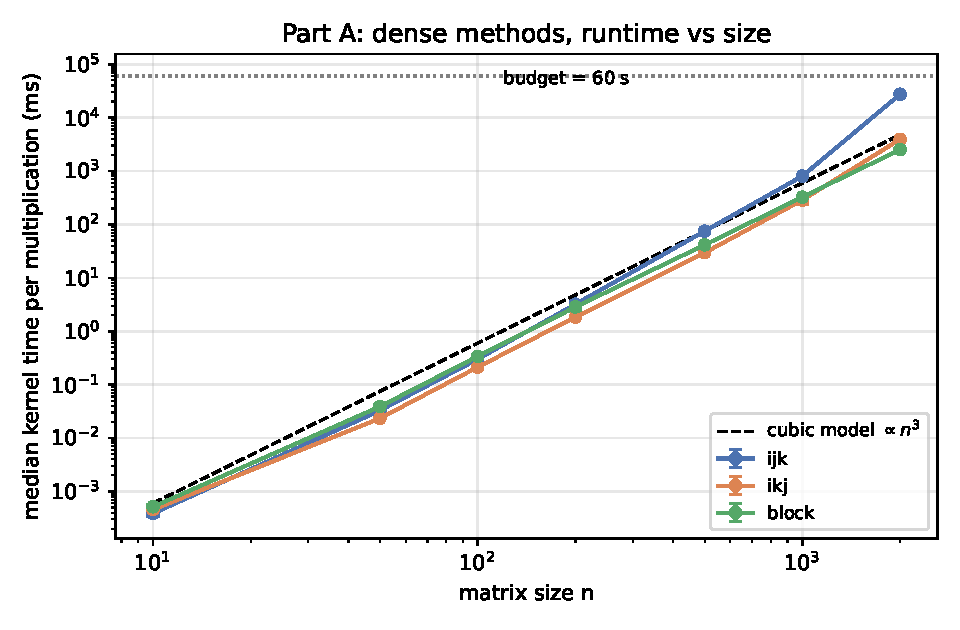
\includegraphics[width=0.95\linewidth]{fig1_runtime_loglog.pdf}
\caption{Median kernel time per multiplication versus matrix size (log--log,
IQR error bars) against the $n^3$ reference line. The dotted line is the 60\,s
budget; timeout configurations are annotated but not plotted, because assigning
them a runtime would fabricate data. Python follows a parallel line about two
orders of magnitude above C; Java and C converge towards the cubic reference at
small $n$ and bend above it from $n=500$.}
\label{fig:scaling}
\end{figure}

Fitting $\log T = a + p \log n$ by ordinary least squares over the sizes
$n \ge 100$ (smaller sizes are dominated by fixed call overheads) gives the
exponents in Table~\ref{tab:fit}; all fits are close to $p = 3$ but systematically
above it, with $R^2 \ge 0.995$.

\begin{table}[htbp]
\centering
\caption{Fitted growth exponents over $n \ge 100$ (hypothesis H1 predicts $p=3$).}
\label{tab:fit}
\begin{tabular}{@{}lrrr@{}}
\toprule
Language & exponent $p$ & $R^2$ & sizes used \\
\midrule
Python & 3.223 & 0.9998 & 100, 200, 500 \\
Java   & 3.640 & 0.9952 & 100, 200, 500, 1000 \\
C      & 3.366 & 1.0000 & 100, 200, 500, 1000 \\
\bottomrule
\end{tabular}
\end{table}

The constant factors (hypothesis H2) are summarised in
Figure~\ref{fig:relative}: Python is 113--169$\times$ slower than C and
40--102$\times$ slower than Java over the shared feasible range; Java is
1.2--2.9$\times$ slower than C. Peak throughput reaches 2.46\,GFLOP/s (C,
$n=50$), 1.49\,GFLOP/s (Java, $n=50$) and 0.015\,GFLOP/s (Python, $n=50$),
against the 8.6\,GFLOP/s peak a 2.8\,GHz core could theoretically sustain with one
multiply--add per cycle; the decline of all three curves at large $n$ reflects
memory-bandwidth and cache-miss costs rather than the arithmetic.

\begin{figure}[htbp]
\centering
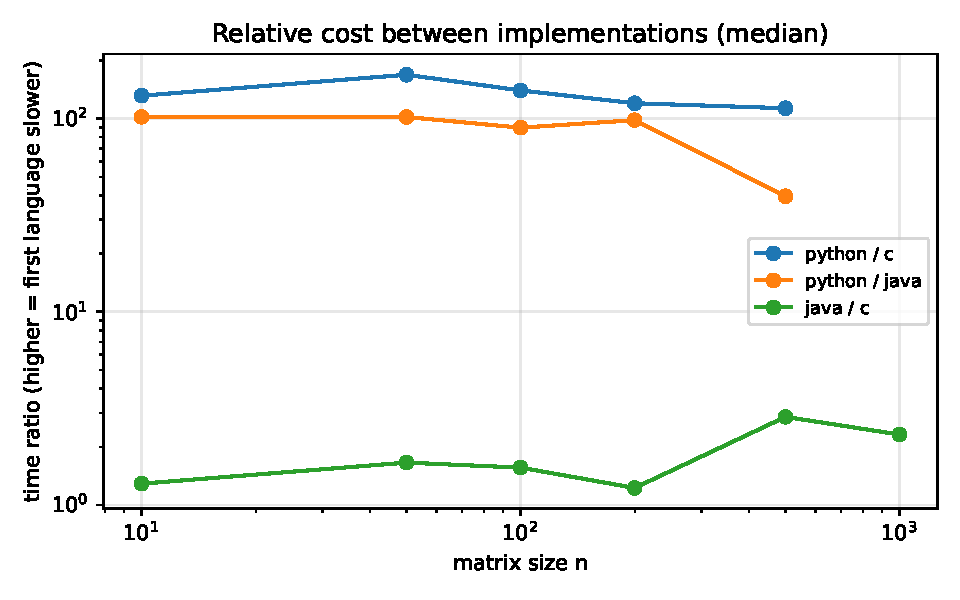
\includegraphics[width=0.95\linewidth]{fig2_relative_speed.pdf}
\caption{Ratio of median times between implementations at shared sizes (log--log).
Ratios are roughly constant in the cache-resident regime; the Java/C ratio rises
above $n=200$ as Java's larger memory footprint and GC activity accumulate, while
Python's gap to C slowly narrows (169$\times$ at $n=50$ to 113$\times$ at $n=500$)
because fixed per-call overheads inflate the very small sizes.}
\label{fig:relative}
\end{figure}

\subsection{Variability}

Figure~\ref{fig:variability} shows the IQR as a percentage of the median and the
full distribution of the five samples. Most configurations are stable
(IQR $\le 5\,\%$); the exception is Java at $n=500$ (IQR 36.5\,\%), which coincided
with the highest background CPU activity of the campaign, and Python at $n=500$
(10.2\,\%). No sample was discarded; the median is robust to these bursts.

\begin{figure}[htbp]
\centering
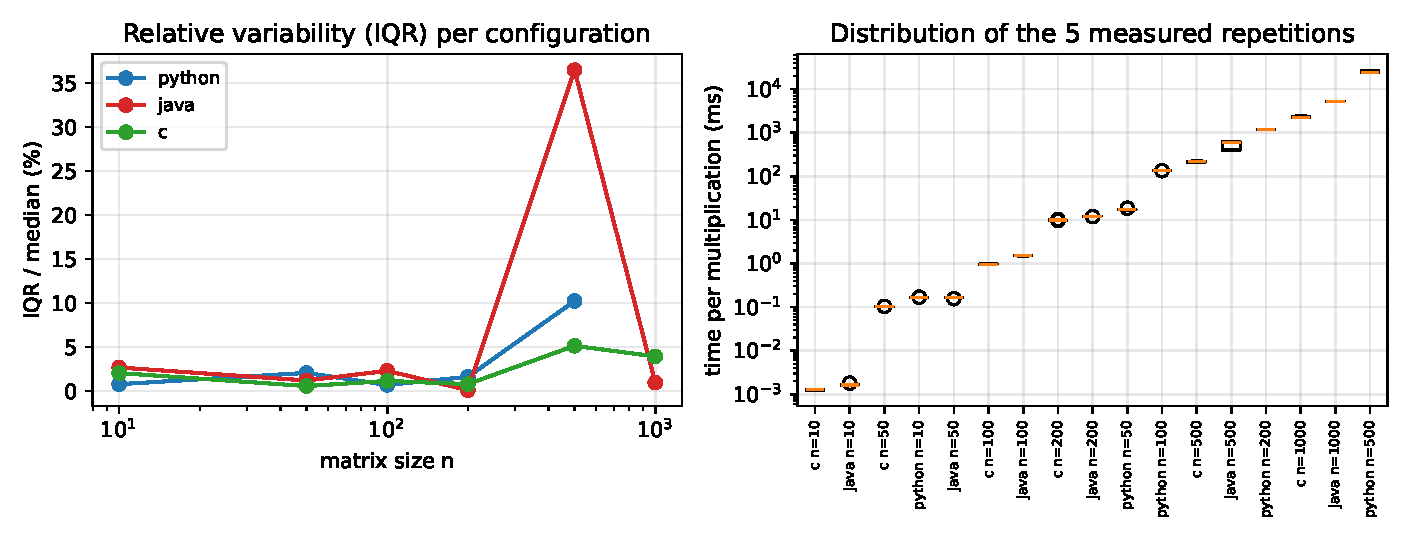
\includegraphics[width=0.98\linewidth]{fig3_variability.pdf}
\caption{Left: IQR of the five repetitions relative to the median, per
configuration. Right: box plot of the same samples (log scale). The spread
measures machine noise (background desktop load, frequency scaling), not
algorithmic variance, because each configuration is deterministic.}
\label{fig:variability}
\end{figure}

\subsection{Memory}

Table~\ref{tab:mem} reports peak resident memory (the named metric of this study).
C tracks the $24n^2$-byte model plus a few megabytes of process overhead;
Python adds about 16--20\,MB of interpreter baseline; Java carries a
$\sim$40\,MB JVM baseline that grows to 106\,MB at $n=1000$ (heap plus JIT code,
class metadata and threads). This supports H3: quadratic growth plus a constant
per-language overhead. The theoretical raw storage is 6\,MB at $n=500$ and 24\,MB
at $n=1000$.

\begin{table}[htbp]
\centering
\caption{Peak process resident memory in MB (psutil, 50\,ms sampling). ``--'' =
configuration not run (budget exceeded).}
\label{tab:mem}
\begin{tabular}{@{}lrrr@{}}
\toprule
$n$ & Python & Java & C \\
\midrule
10   & 18 & 74 & 4 \\
50   & 16 & 42 & 4 \\
100  & 20 & 43 & 4 \\
200  & 21 & 46 & 5 \\
500  & 46 & 54 & 10 \\
1000 & -- & 106 & 27 \\
2000 & -- & -- & -- \\
\bottomrule
\end{tabular}
\end{table}

\begin{figure}[htbp]
\centering
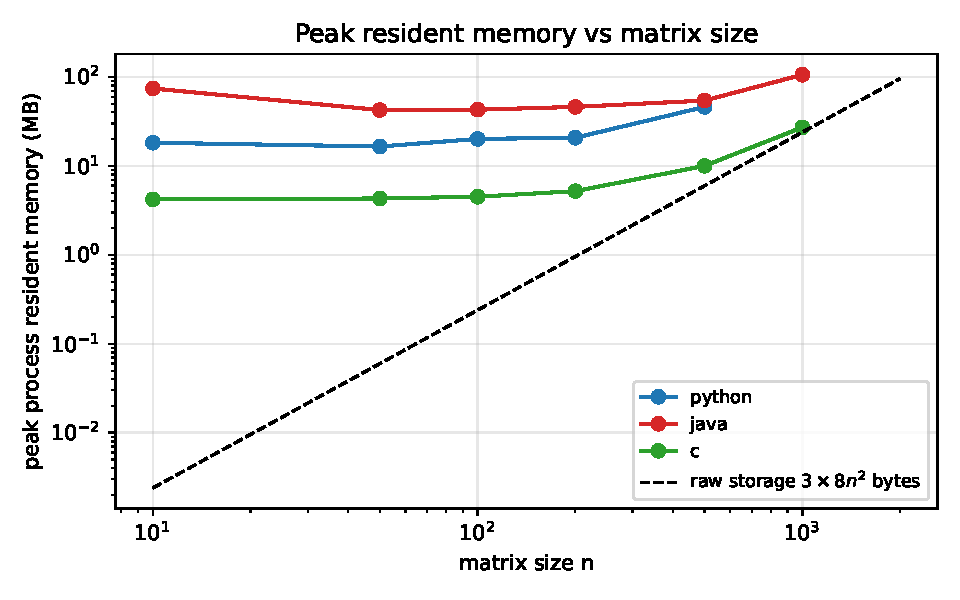
\includegraphics[width=0.95\linewidth]{fig4_memory.pdf}
\caption{Peak resident memory versus $n$ (log--log) against the raw-storage line
$3 \times 8n^2$ bytes. The vertical offset of each curve is the runtime overhead
of the language; the slopes match the quadratic model at large $n$.}
\label{fig:memory}
\end{figure}

\subsection{Warm-up effect (Java)}

Figure~\ref{fig:warmup} replays the excluded warm-up kernels of the Java $n=10$
run: the first multiplication of a fresh JVM takes 62.5\,$\mu$s (mostly
interpreted), while the steady state is 2.10\,$\mu$s -- a $30\times$ difference
inside a single process. Including warm-ups would have biased every Java number
upwards; excluding them, as the protocol requires, does not hide compilation cost
but reports the steady-state behaviour that the other two languages exhibit from
their first call.

\begin{figure}[htbp]
\centering
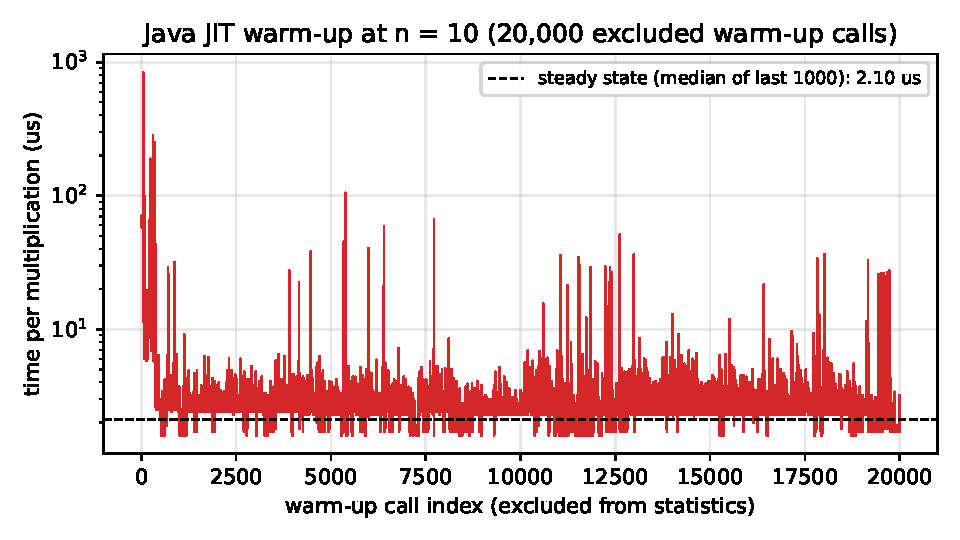
\includegraphics[width=0.95\linewidth]{fig5_java_warmup.pdf}
\caption{Java per-call time during the 20\,000 excluded warm-up calls at $n=10$
(log scale). Spikes are JIT recompilation and garbage-collection pauses; the
dashed line marks the steady-state median of the last 1000 calls (2.10\,$\mu$s).}
\label{fig:warmup}
\end{figure}

\subsection{Limits under the declared budgets}

\begin{table}[htbp]
\centering
\caption{Feasibility limits (budget: 60\,s per multiplication, 4\,GiB memory).}
\label{tab:limits}
\begin{tabular}{@{}llll@{}}
\toprule
Language & Largest feasible $n$ (median) & Over budget & Killed before 1st kernel \\
\midrule
Python & 500 (24.2\,s) & -- & 1000, 2000 \\
Java   & 1000 (5.2\,s) & -- & 2000 \\
C      & 1000 (2.3\,s) & 2000 (probe: 77.0\,s, 75.9\,s) & -- \\
\bottomrule
\end{tabular}
\end{table}

Python at $n=1000$ and both Python and Java at $n=2000$ were terminated by the
150\,s probe deadline before the first kernel completed, so no runtime exists for
them. C at $n=2000$ completed its probe twice (77.0\,s and 75.9\,s, consistent to
1.4\,\%) and therefore is a measured \emph{over-budget} result: the memory
hierarchy at 96\,MB of working matrices pushes the naive kernel past the budget
even in native code. All four timeout outcomes are results in themselves: they
locate the feasibility frontier required by the assignment.

\section{Discussion}
\label{sec:discussion}

\textbf{Answer to the research question.} Within the tested scope, size affects
runtime cubically with language-specific constants: over $n \ge 100$ the fitted
exponents are 3.22 (Python), 3.64 (Java) and 3.37 (C), all close to the
algorithmic $n^3$ model but above it because the working set outgrows the caches.
Python pays a 113--169$\times$ constant relative to C (interpreted dispatch and
boxed floats), Java only 1.2--2.9$\times$ after JIT compilation. Memory grows
quadratically plus a constant runtime overhead (H3 confirmed: C $\approx 24n^2$ +
4\,MB, Python + 16\,MB, Java + 42\,MB).

\textbf{Why the exponents exceed three.} Between $n=500$ and $n=1000$ C grows
$10.6\times$ instead of $8\times$: $B$ grows from 2\,MB (fits the last-level
cache) to 8\,MB and the $B$-column access stride doubles to 8\,kB, increasing
cache and TLB misses -- a memory-system effect, not an algorithmic one. Java's
larger exponent (3.64) includes GC and heap effects and the noisy $n=500$ point
(IQR 36.5\,\%).

\textbf{Why the curves are not perfectly parallel.} Small sizes are inflated by
fixed costs that differ per language (function-call and interpreter overheads are
large relative to $n=10$ work), so ratios drift: Python/C falls from 131$\times$
at $n=10$ to 113$\times$ at $n=500$ while Java/C rises from 1.29 to 2.85 as
Java's footprint grows.

\textbf{Limitations.}
\begin{enumerate}
  \item \textbf{Shared, uncontrolled machine:} background load averaged 24\,\%
        (max 100\,\%) during the campaign; the largest observed IQR is 36.5\,\%.
        Medians with five samples mitigate but cannot eliminate this noise.
        The campaign could be repeated on an idle or pinned system.
  \item \textbf{Single machine, single input set, single seed:} results do not
        generalise to other hardware, value distributions or $m \ne n$ shapes.
  \item \textbf{Compiler settings:} GCC \texttt{-O2} may auto-vectorise the C
        kernel with the default x86-64 SSE2 target; this is fixed and documented,
        and it is one reason the C constant is small. It does not change the
        algorithmic complexity.
  \item \textbf{Metric heterogeneity:} peak resident memory, managed heap and raw
        array storage are distinct quantities and are reported as such.
  \item \textbf{Timeouts:} for killed probes no runtime exists; none was
        interpolated from smaller sizes.
\end{enumerate}
Following the assignment guidance, no claim is made that one language is
universally faster; the comparison is scoped to these implementations, flags,
inputs and hardware~\cite{fleming1986,mytkowicz2009}.

\section{Conclusions}

Within the tested scope the study establishes that: (1) the basic $O(n^3)$
triple-loop multiplication grows close to cubically in all three languages
($p = 3.22$--$3.64$ for $n \ge 100$), with super-cubic deviations appearing once
the matrices leave the last-level cache; (2) language constants dominate the
absolute times -- Python 113--169$\times$ C, Java 1.2--2.9$\times$ C -- while
Java's JIT warm-up is a real, measurable effect that must be excluded from steady
state; (3) peak resident memory follows $24n^2$ bytes plus a constant runtime
overhead; and (4) under a 60\,s budget the largest feasible sizes are $n=500$
(Python) and $n=1000$ (Java, C), with $n=2000$ exceeding the budget in all three
languages -- in C a measured 76\,s, in Python and Java a deadline kill without a
runtime.

What remains unresolved: behaviour on an idle or pinned system, other value
distributions and rectangular shapes, and the optimisation questions (blocking,
loop reordering, sparse storage) that Assignment~2 addresses.

\section{Reproducibility materials}

{\sloppy
All source code, shared inputs, raw measurements (CSV) and the executed analysis
notebook live in the public repository
\url{https://github.com/aledelgadoo/individual-assignments-bigdata};
the Git tag \texttt{assignment-1} marks the exact state submitted for this
assignment. The repository's \texttt{README.md} documents the dependency
versions and the exact build, run and analysis commands that regenerate this
report end to end.\par}

\section*{Generative-AI usage statement}

Following the course policy, the author discloses that the AI assistant
\textbf{opencode} (model \texttt{opencode/mimo-v2.6-flash-free}) was used, under
the author's direction, for planning the measurement harness, drafting and
debugging parts of the scripts, generating the analysis notebook and figures, and
revising the English of this report. The author reviewed all generated code,
executed and inspected the correctness tests, the benchmark campaign and every
figure, verified the numbers quoted here against the raw CSV files, and is
responsible for the measurements, the conclusions and any errors.

\begin{thebibliography}{9}
\bibitem{strang2016}
G. Strang, \emph{Introduction to Linear Algebra}, 5th ed.
Wellesley--Cambridge Press, 2016.

\bibitem{cormen2022}
T. H. Cormen, C. E. Leiserson, R. L. Rivest, and C. Stein,
\emph{Introduction to Algorithms}, 4th ed. MIT Press, 2022.

\bibitem{fleming1986}
W. P. Fleming and J. M. Wallace, ``How not to lie with statistics: the correct
way to summarize benchmark results,'' \emph{Communications of the ACM},
vol. 29, no. 3, pp. 218--221, 1986.

\bibitem{mytkowicz2009}
T. Mytkowicz, A. Diwan, M. W. Hauswirth, and P. F. Sweeney,
\emph{Measuring Computer Performance: A Practitioner's Guide}.
Cambridge University Press, 2009.

\bibitem{jvms21}
Oracle, ``The Java Virtual Machine Specification, Java SE 21 Edition,'' 2023.
[Online]. Available:
\url{https://docs.oracle.com/javase/specs/jvms/se21/html/}

\bibitem{pythonfloat}
Python Software Foundation, ``Built-in types --- float,'' \emph{Python Language
Reference}, 2024. [Online]. Available: \url{https://docs.python.org/3/library/float.html}

\bibitem{isoC11}
ISO/IEC 9899:2011, ``Information technology --- Programming languages --- C,''
International Organization for Standardization, 2011.

\bibitem{psutil}
G. Rodola, \emph{psutil: cross-platform process and system utilities},
2024. [Online]. Available: \url{https://psutil.readthedocs.io/}

\bibitem{intelark}
Intel, ``Intel Core i7-1355U Processor,'' Intel ARK product database.
[Online]. Available: \url{https://ark.intel.com/}
\end{thebibliography}

\end{document}
